\everymath{\displaystyle}
\documentclass{beamer}
% \documentclass[handout]{beamer}

%\usepackage[pdftex]{color,graphicx}
\usepackage{amsmath,amssymb,amsfonts}

\mode<presentation>
{
  % \usetheme{Darmstadt}
  % \usetheme[hideothersubsections]{Hannover}
  % \usetheme[hideothersubsections]{Goettingen}
  \usetheme[hideothersubsections, right]{Berkeley}

  \usecolortheme{seahorse}
  % \usecolortheme{dolphin}
  \usecolortheme{rose}
  % \usecolortheme{orchid}

  \useinnertheme[shadow]{rounded}

  \setbeamercovered{transparent}
  % or whatever (possibly just delete it)
}

\mode<handout>{
  \setbeamercolor{background canvas}{bg=black!5}
  \usepackage{pgfpages}
  \pgfpagesuselayout{4 on 1}[a4paper,border shrink=5mm, landscape]
}

\usepackage[brazilian]{babel}
% or whatever

% \usepackage[latin1]{inputenc}
\usepackage[utf8]{inputenc}
% or whatever

\usepackage{times}
%\usepackage[T1]{fontenc}
% Or whatever. Note that the encoding and the font should match. If T1
% does not look nice, try deleting the line with the fontenc.


\title%[] % (optional, use only with long paper titles)
{Introdução}

\subtitle
{Conhecimento} % (optional)

\author%[] % (optional, use only with lots of authors)
{Felipe Figueiredo}% \and S.~Another\inst{2}}
% - Use the \inst{?} command only if the authors have different
%   affiliation.

\institute[INTO] % (optional, but mostly needed)
{Instituto Nacional de Traumatologia e Ortopedia
}
  % \inst{1}%
  % Department of Computer Science\\
  % University of Somewhere
  % \and
  % \inst{2}%
  % Department of Theoretical Philosophy\\
  % University of Elsewhere}
% - Use the \inst command only if there are several affiliations.
% - Keep it simple, no one is interested in your street address.

\date%[] % (optional)
{}

% \subject{Talks}
% This is only inserted into the PDF information catalog. Can be left
% out. 



% If you have a file called "university-logo-filename.xxx", where xxx
% is a graphic format that can be processed by latex or pdflatex,
% resp., then you can add a logo as follows:

\pgfdeclareimage[height=1.6cm]{university-logo}{../logo}
\logo{\pgfuseimage{university-logo}}



% Delete this, if you do not want the table of contents to pop up at
% the beginning of each subsection:
\AtBeginSubsection[]
%\AtBeginSection[]
{
  \begin{frame}<beamer>{Sumário}
    \tableofcontents[currentsection,currentsubsection]
  \end{frame}
}


% If you wish to uncover everything in a step-wise fashion, uncomment
% the following command: 

\beamerdefaultoverlayspecification{<+->}


\begin{document}

\begin{frame}
  \titlepage
\end{frame}

\begin{frame}{Sumário}
  \tableofcontents
  % You might wish to add the option [pausesections]
\end{frame}


%% Template
% \section{}

% \subsection{}

% \begin{frame}{}
%   \begin{itemize}
%   \item 
%   \end{itemize}
% \end{frame}

% \begin{frame}
%   \begin{columns}
%     \begin{column}{5cm}
%     \end{column}
%     \begin{column}{5cm}
%     \end{column}
%   \end{columns}
% \end{frame}

% \begin{frame}{}
%   \includegraphics[height=0.4\textheight]{file1}
%   \includegraphics[height=0.4\textheight]{file2}
%   \includegraphics[height=0.4\textheight]{file3}
%   \begin{figure}
%     \caption{}
%   \end{figure}
% \end{frame}

% \begin{frame}{}
%   \begin{definition}
%   \end{definition}
%   \begin{example}
%   \end{example}
%   \begin{block}{Exercício}
%   \end{block}
% \end{frame}

\section{A disciplina}

\subsection{Apresentação}

\begin{frame}{Docente}
Felipe Figueiredo

\bigskip

Email:

\href{mailto:prof.felipefigueiredo@gmail.com}{prof.felipefigueiredo@gmail.com}

\bigskip

Página:

\href{http://sites.google.com/site/proffelipefigueiredo}{http://sites.google.com/site/proffelipefigueiredo}

\end{frame}

\subsection{Disciplina}

\begin{frame}{Objetivos}
Oferecer uma introdução suave a
  \begin{itemize}
  \item Metodologia científica
  \item Redação científica
  \end{itemize}
\end{frame}

\begin{frame}{Bibliografia}
  \begin{itemize}
  \item {\bf Fundamentos de Metodologia Científica} (Eva Maria Lakatos
    e Marina de Andrade Marconi)
  \item Outros materiais online linkados na página da disciplina.
  \end{itemize}
\end{frame}

\begin{frame}{O que esperar da disciplina}
  \begin{enumerate}
  \item<2-> \alert<2>{Introdução: conhecimento} (cap 3)
  \item<2-> \alert<2>{Métodos científicos} (cap 4)
  \item<2-> \alert<2>{Hipóteses, variáveis} (caps 6,7)
  \item<2-> \alert<2>{Pesquisa bibliográfica e resumo} (cap 2)
  \item<3-> \alert<3>{Planejamento} (cap 8)
  \item<3-> \alert<3>{EDA}
  \item<3-> \alert<3>{Desenho experimental}
  \item<4-> \alert<4>{Projeto I - Projeto e relatório} (cap 10)
  \item<4-> \alert<4>{Projeto II - Dissertação e artigos} (caps 11,12)
  \item<4-> \alert<4>{Citações, Referências e Plágio} (cap 13)
  \item<5-> \alert<5>{Tópicos de escrita científica} (Gopen, Swan)
  \item<6-> \alert<6>{Indicadores em Ciência} (Hirsch)
  \item<1-> Seminários
  \item<1-> Seminários
  \item<1-> Seminários
  \end{enumerate}
\end{frame}

\begin{frame}{Avaliação}
  \begin{itemize}
  \item Escrita de um projeto {\em ad-hoc}.
  \item Seminário de defesa do projeto.
  \end{itemize}
\end{frame}

\section{Conhecimento}

\subsection{Conceitos preliminares}

% \subsection{Verdade}

\begin{frame}{Verdade}
  \begin{columns}
    \begin{column}{6cm}<1-> ``{\em When you have eliminated the
        impossible, whatever remains, however improbable, must be the
        truth.}'' Sherlock Holmes
    \end{column}
    \begin{column}{4cm}<1->
      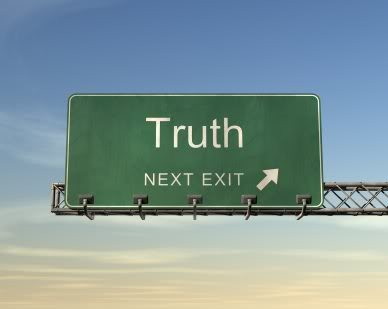
\includegraphics[height=0.4\textheight]{truth}
    \end{column}
  \end{columns}
\end{frame}

% \subsection{Evidências}

\begin{frame}{Evidências}
  ``{\em It is a capital mistake to theorize before one has
    data. Insensibly one begins to twist facts to suit theories,
    instead of theories to suit facts.}'' Sherlock Holmes
\end{frame}

% \subsection{Dados, Informação e Conhecimento}

\begin{frame}{Dados, Informação e Conhecimento}
  \begin{itemize}
  % \item ``Evidence-based medicine (EBM) is the process of
  %   systematically reviewing, appraising and using clinical research
  %   findings to aid the delivery of optimum clinical care to
  %   patients''
  \item Dados: elementos, códigos ou símbolos quantificáveis que são
    coletados em um experimento.
  \item Informação: agregração e interpretação de dados
  \item Conhecimento: agregação de um corpo de informações que tem
    significado e aplicabilidade prática
  \end{itemize}
\end{frame}


\begin{frame}{Dados, Informação e Conhecimento}
  \begin{center}
    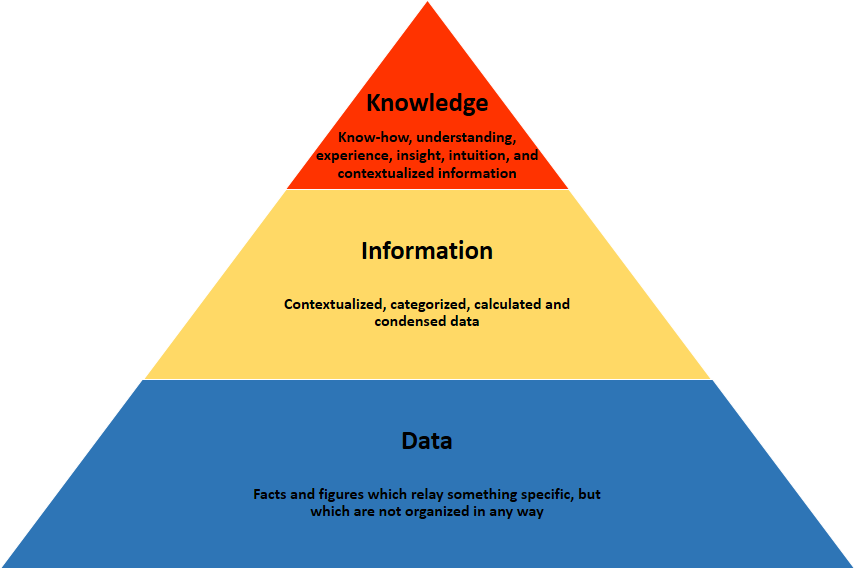
\includegraphics[height=0.9\textheight]{Knowledge_pyramid}
  \end{center}
  % \begin{figure}
  %   \caption{}
  % \end{figure}
\end{frame}

% \begin{frame}{Dados, Informação e Conhecimento}
%   \begin{example}
%     Dados do mercado financeiro: preço das ações da Petrobrás hoje
%   \end{example}
% \end{frame}

\subsection{Tipos de conhecimento}

% \subsection{Conhecimento Popular}

\begin{frame}{Conhecimento Popular}
  \begin{itemize}
  \item Senso comum
  \item Subjetivo
  \item 
  \end{itemize}
\end{frame}

% \subsection{Conhecimento Teológico}

\begin{frame}{Conhecimento Teológico}
  \begin{itemize}
  \item 
  \end{itemize}
\end{frame}

% \subsection{Conhecimento Filosófico}

\begin{frame}{Conhecimento Filosófico}
  \begin{itemize}
  \item 
  \end{itemize}
\end{frame}

% \subsection{Conhecimento Científico}

\begin{frame}{Conhecimento Científico}
  \begin{itemize}
  \item 
  \end{itemize}
\end{frame}


\subsection{Resumo}

\begin{frame}{Senso Comum x Conhecimento Científico}
  \begin{itemize}
  \item 
  \end{itemize}
\end{frame}


\end{document}
